\id{МРНТИ 65.09.03}
\end{minipage} \\
\midrule\noalign{}
\endhead
\bottomrule\noalign{}
\endlastfoot
\end{longtable}

{\bfseries ӨСІМДІК ТЕКТЕС АНТИОКСИДАНТТАРДЫ ҚОЛДАНУ АРҚЫЛЫ ЙОГУРТ
ТЕХНОЛОГИЯСЫН ЖАСАУ}

\begin{figure}[H]
	\centering
	
\includegraphics[width=0.8\textwidth]{media/pish3/image1}
	\caption*{}
\end{figure}

\textsuperscript{1}Б.
\begin{figure}[H]
	\centering
	
\includegraphics[width=0.8\textwidth]{media/pish3/image1}
	\caption*{}
\end{figure}

\begin{figure}[H]
	\centering
	
\includegraphics[width=0.8\textwidth]{media/pish3/image1}
	\caption*{}
\end{figure}


\emph{\textsuperscript{1}С.Сейфуллин атындағы Қазақ агротехникалық
университеті, Астана, Қазақстан,}

\emph{\textsuperscript{2}Қ. Құлажанов атындағы Қазақ технология және
бизнес университеті, Астана, Қазақстан}

{\bfseries \textsuperscript{\envelope }}Автор-корреспондент: nurmashanova@gmail.com

Йогурт өндірісінде бұрын қолданылмаған өсімдік тектес жаңа
компоненттерді пайдалану өнімге тек мүлдем жаңа дәмдік қасиеттер беріп
қана қоймай, сонымен қатар оны адам ағзасына қажетті маңызды
нутриенттермен байытып, функционалдық мақсаттағы тағам өнімін әзірлеуге
мүмкіндік береді.Осы зерттеудің мақсаты -- функционалды сүтқышқылды
өнімдер дайындауда қызылша ұнтағын байытқыш ретінде қолданудың әсерін
зерттеу болды. Жұмыс барысында әртүрлі концентрациядағы өсімдік қоспасы
ретінде қызылша ұнтағы қосылған сүтқышқылды йогурттың үлгілері
дайындалды. Қызылша ұнтағы пастеризацияланған сүтке қосылып, сүтқышқылды
бактерияларды қоспастан бұрын араластырылды. Зерттеу нәтижесінде қызылша
ұнтағын байытқыш ретінде пайдалану сүт қышқылын ашыту уақытын қысқартуға
мүмкіндік беретіндігі анықталды. Алынған йогурт үлгілерінің сапасы
органолептикалық, физика-химиялық көрсеткіштер бойынша бағаланып,
дәмсараптау сынақтары жүргізілді. Қосылған өсімдік қоспасының йогурттың
сыртқы түріне, құрылымына, дәміне оң әсер еткендігі анықталды. Қызылша
ұнтағын қосу сүттің суспензиясын азайтып, йогурттың су байланыстыру
қабілетін арттырды. Алынған йогурт үлгілерінің тағамдық құндылығы
есептеліп, 0,25\% қызылша ұнтағы қосылған үлгіде темірдің мөлшерінің
артқаны анықталды.

{\bfseries Түйін сөздер:} функционалды тағамдар, йогурт, сүтқышқылды өнім,
антиоксидант, қызылша ұнтағы, сапасын бағалау.

{\bfseries РАЗРАБОТКА ТЕХНОЛОГИИ ЙОГУРТА С ИСПОЛЬЗОВАНИЕМ АНТИОКСИДАНТОВ
РАСТИТЕЛЬНОГО ПРОИСХОЖДЕНИЯ}

{\bfseries \textsuperscript{1}Н.С. Машанова, \textsuperscript{1}Б.
Калемшарив, \textsuperscript{1}А.С. Жолшиева, \textsuperscript{2}А.А.
Бектурганова}

\emph{{\bfseries \textsuperscript{1}}Казахский агротехнический университет
им. С.Сейфуллина, Астана, Казахстан,}

\emph{\textsuperscript{2}Казахский университет технологии и бизнеса им
К.Кулажанова, Астана, Казахстан,}

\emph{e-mail: nurmashanova@gmail.com}

Использование новых компонентов растительного происхождения, ранее не
применявшихся при производстве йогурта, не только придает продукту
совершенно новые вкусовые свойства, но и обогащает его важными
питательными веществами, необходимыми для организма человека, что
позволяет разрабатывать функциональные продукты питания. Целью данного
исследования было изучение влияния использования порошка свеклы в
качестве обогатителя при приготовлении функциональных молочнокислых
продуктов. В ходе работы были приготовлены образцы кисломолочного
йогурта с добавлением в качестве растительной добавки порошка свеклы в
различных концентрациях. Свекольный порошок добавляли в пастеризованное
молоко и перемешивали перед добавлением молочнокислых бактерий.
Исследование показало, что использование порошка свеклы в качестве
обогатителя может сократить время, необходимое для ферментации молочной
кислоты. Качество полученных образцов йогурта оценивали по
органолептическим, физико-химическим показателям, проводили
дегустационные испытания. Установлено, что добавленная растительная
смесь оказала положительное влияние на внешний вид, текстуру и вкус
йогурта. Добавление свекольного порошка уменьшило взвесь молока и
увеличило водосвязывающую способность йогурта. Была рассчитана пищевая
ценность полученных образцов йогурта и установлено, что содержание
железа в образце увеличилось при добавлении 0,25\% свекольного порошка.

{\bfseries Ключевые слова:} функциональные продукты питания, йогурт,
молочнокислый продукт, антиоксидант, свекольный порошок, оценка
качества.

{\bfseries DEVELOPMENT OF YOGURT TECHNOLOGY WITH PLANT-BASED ANTIOXIDANTS}

{\bfseries \textsuperscript{1}N.S. Mashanova, \textsuperscript{1}B.
Kalemshariv, \textsuperscript{1}A.S. Zholshieva, \textsuperscript{2}A.A.
Bekturganova}

\emph{{\bfseries \textsuperscript{1}}Kazakh Agrotechnical University named
after S.Seifullin, Astana, Kazakhstan,}

\emph{\textsuperscript{2}Kazakh University of Technology and Business
named after K.Kulazhan,}

\emph{Astana, Kazakhstan,}

\emph{e-mail: nurmashanova@gmail.com}

The use of new components of plant origin, previously unused in yogurt
production, not only gives the product completely new taste properties,
but also enriches it with important nutrients necessary for the human
body, allowing the development of functional food products. The purpose
of this study was to study the effect of using beetroot powder as a
fortifier in the preparation of functional lactic acid products. During
the work, samples of lactic acid yogurt with beetroot powder as a plant
additive in various concentrations were prepared. Beetroot powder was
added to pasteurized milk and mixed before adding lactic acid bacteria.
As a result of the study, it was found that using beetroot powder as an
fortifier allows you to reduce the time of lactic acid fermentation. The
quality of the obtained yogurt samples was evaluated according to
organoleptic, physicochemical indicators, and taste tests were
conducted. It was found that the added plant additive had a positive
effect on the appearance, structure, and taste of yogurt. The addition
of beetroot powder reduced the suspension of milk and increased the
water-binding capacity of yogurt. The nutritional value of the obtained
yogurt samples was calculated, and it was found that the iron content
increased in the sample with the addition of 0.25\% beetroot powder.

{\bfseries Keywords:} functional foods, yogurt, lactic acid product,
antioxidant, beetroot powder, quality assessment.

{\bfseries Кіріспе.} Тағам өнімдерінің ішінде сүт өнімдері жеке адамдардың
рационында маңызды орын алады, ал өндірушілер денсаулыққа пайдалы сүт
өнімдерін жасау бойынша айтарлықтай қадамдар жасауда, сондықтан
байытылған сүт өнімдерін тұтыну соңғы уақытта артып келеді. Йогурт --
сүттің бактериялық ашытуы арқылы алынатын өнім {[}1{]}.

Соңғы уақытта тұтынушылардың пайдалы тағамдарға деген қызығушылығы
маңызды қоректік заттарды қамтамасыз ететін және адамның денсаулығына оң
әсер ететін функционалды тағамдардың өндірісіне алып келді. Функционалды
тағамдар табиғи немесе өңделген тағамдар ретінде анықталады, олардың
құрамында белгілі немесе белгісіз биологиялық белсенді қосылыстар бар
және олар белгілі бір мөлшерде қолданғанда клиникалық дәлелденген
денсаулыққа пайдалы әсер етеді, соның ішінде созылмалы аурулардың алдын
алу, басқару немесе емдеу {[}2{]}. Осылайша, функционалды тағамдардың
ішінде йогурттың ерекше орны бар, өйткені оның құрамындағы сүт қышқылы
бактериялары мен пробиотиктер адам денсаулығына пайдалы әсер етіп, ас
қорыту жүйесін қолдауға көмектеседі, сонымен қатар сүйектер мен
тістердің саулығын қамтамасыз етеді.

Қазіргі замандағы өмір салты, химиялық заттарға ұшырау, қоршаған ортаның
ластануы, темекі шегу, дәрі-дәрмектер, аурулар және стресс сияқты
факторлар оксидативті стреске байланысты аурулардың пайда болу қаупін
арттырады. Өсімдік, жануар және минерал көздерінен алынатын
антиоксиданттарды тұтыну адам денсаулығына пайдалы екені дәлелденген,
сонымен қатар олар еркін радикалдардың әсерінен туындайтын аурулардың
алдын алуда тиімді болып табылады. Антиоксиданттар еркін радикалдардың
түзілуін азайтуға көмектеседі және науқастардың антиоксиданттық статусын
жақсартады, сондықтан оларды тұтыну қалыпты ағзалық қызметті қалпына
келтіруге және осындай ауруларды емдеуге оң әсерін тигізуі
мүмкін.Антиоксиданттардың денсаулыққа пайдалы әсері мен йогурттың
сапасын жақсартуға бағытталған қоспалар арасындағы байланыс, олардың
екеуінің де ағзадағы табиғи процестерді қолдауға және аурулардың алдын
алуға, сонымен қатар өнімнің сапасын арттыруға көмектесетінімен
ерекшеленеді.

Антиоксиданттарды тағам өндірісінде, әсіресе, сүт өнімдерінде,
шырындарда, консервіленген тағамдарда кеңінен қолданады. Олар өнімдердің
сақтау мерзімін ұзартуға, дәмін жақсартуға және олардың қоректік
құндылығын арттыруға көмектеседі {[}3{]}.

Денсаулық сақтаушысы антиоксиданттардың көптеген тағамдарда
кездесетініне табиғатқа алғыс айтуымыз керек. Олардың көпшілігі белгілі
С, Е және А дәрумендері, сондай-ақ бета-каротин және полифенолдар
{[}4{]}.

Тағамдар мен дәрілік өсімдіктерден антиоксиданттарды тиімді алу және
дұрыс бағалау антиоксиданттардың әлеуетті көздерін зерттеу және оларды
функционалды тағамдарда, фармацевтикада және диеталық қоспаларда
қолдануды ілгерілету үшін өте маңызды {[}5{]}.

Сүт өнімдерінде табиғи антиоксиданттарды қолдану ғылыми зерттеулерде
ұзақ тарихы бар, және қазіргі таңда да тағам ғылымының ғалымдарының
назарын аударып келеді {[}6{]}.

Йогурт сапасын жақсарту және сақтау мерзімін ұзарту үшін оған
синтетикалық (мысалы, аспартам тәттілендіргіші) немесе табиғи (мысалы,
пектин қоюлатқышы, ол алма мен цитрусты жемістердің қабығында болады)
қоспалар қосылады. Йогурт өндірісінде жиі қолданылатын тағамдық
қоспаларға эмульгаторлар, қоюлатқыштар, хош иістендіргіштер, бояғыштар,
тәттілендіргіштер, қышқылдық реттегіштер және консерванттар жатады.

Осыған балама ретінде өсімдік негізіндегі табиғи биоактивті қоспаларды
(NPBH) қолдану мүмкіндігі зерттелуде. Бұл әдісте өсімдік тіндері
ұнтақталып, араластырылып, олардың құрамындағы пайдалы компоненттер
сақталады. Мұндай қоспаларды йогуртқа қосу оның құрылымын жақсартып, су
ұстап тұру және гель түзу қасиеттерін арттырады. Сондықтан, химиялық
синтезделген қоспалардың орнына табиғи өсімдік

текті қоспаларды қолдану -- йогурт өндірісінде тиімді әрі қауіпсіз әдіс
болуы мүмкін {[}7{]} .

{\bfseries 1- кесте.Өсімдік тектес өнімдердің химиялық құрамын салыстыру}

% \begin{longtable}[]{@{}
%   >{\raggedright\arraybackslash}p{(\columnwidth - 10\tabcolsep) * \real{0.1695}}
%   >{\raggedright\arraybackslash}p{(\columnwidth - 10\tabcolsep) * \real{0.1621}}
%   >{\raggedright\arraybackslash}p{(\columnwidth - 10\tabcolsep) * \real{0.1766}}
%   >{\raggedright\arraybackslash}p{(\columnwidth - 10\tabcolsep) * \real{0.1603}}
%   >{\raggedright\arraybackslash}p{(\columnwidth - 10\tabcolsep) * \real{0.1686}}
%   >{\raggedright\arraybackslash}p{(\columnwidth - 10\tabcolsep) * \real{0.1628}}@{}}
% \toprule\noalign{}
% \begin{minipage}[b]{\linewidth}\raggedright
% Қоректік заттар
% \end{minipage} & \begin{minipage}[b]{\linewidth}\raggedright
% Қызылша
% \end{minipage} & \begin{minipage}[b]{\linewidth}\raggedright
% Қарақат
% \end{minipage} & \begin{minipage}[b]{\linewidth}\raggedright
% Сәбіз
% \end{minipage} & \begin{minipage}[b]{\linewidth}\raggedright
% Қызанақ
% \end{minipage} & \begin{minipage}[b]{\linewidth}\raggedright
% Жүзім
% \end{minipage} \\
% \midrule\noalign{}
% \endhead
% \bottomrule\noalign{}
% \endlastfoot
% су (г) & 87,6 & 83,95 & 8,29 & 94,52 & 80,54 \\
% көмірсу (г) & 9,56 & 15,38 & 9,58 & 3,89 & 18,1 \\
% ақуыз (г) & 1,61 & 1,4 & 0,93 & 0,88 & 0,72 \\
% майлар (г) & 0,17 & 0,41 & 0,24 & 0,2 & 0,16 \\
% с дәрумені (мг) & 4,9 & 181 & 5,9 & 13,7 & 10,8 \\
% темір (мг) & 0,8 & 1,0 & 0,3 & 0,27 & 0,36 \\
% энергия (ккал) & 43 & 63 & 41 & 18 & 69 \\
% \end{longtable}

Йогуртқа қосуға жарамды өсімдік өнімдерін қарастырғанда, олардың
химиялық құрамы, антиоксиданттық белсенділігі және технологиялық
қасиеттері маңызды рөл атқарады. Кестеде көрсетілгендей, йогуртқа қосуға
ең ыңғайлысы - қызылша екенін байқауға болады (1-кесте). Себебі:

- орташа көмірсу мөлшері (9,56г) өнімге тәтті дәм береді;

- ақуыздық құндылығы жоғары (1,61г);

- су мөлшері орташа (87,6г) -- йогурттың консистенциясын өзгертпейді;

- май мөлшері өте аз (0,17г) -- диеталық өнім ретінде пайдалы;

- С дәрумені жеткілікті (4,9мг), темір мөлшері жоғары (0,8мг) -- қан
айналымына пайдалы;

- энергиясы (43ккал) орташа, бұл йогуртың тағамдық құндылығын арттырады.

Осы себептерге байланысты қызылша -- йогуртқа ең қолайлы өнім болып
табылады.

\emph{Қызылша ұнтағы --} табиғи өсімдік тектес қоспа, оның құрамында
биологиялық белсенді заттар мол. Бұл ұнтақ антиоксиданттық қасиетке ие
болып, тағам өнімдерінің қоректік құндылығын арттырады. Қызылша
құрамындағы бетаин мен фенолдық қосылыстар ағзадағы тотығу стрессін
азайтып, жасушаларды қорғайды. Қызылшаның табиғи нитраттардың болуы қан
тамырларын кеңейтіп, жүрек-қан тамыр жүйесіне оң әсер етеді, С дәрумені
мен басқа да фитонутриенттер ағзаның қорғаныс қабілетін күшейтеді.
Қызылшадағы тағамдық талшық ішек микрофлорасын жақсартып, асқорытуды
реттейді.

Зерттеулер көрсеткендей, қызылшаны йогуртқа қосу оның биологиялық
белсенділігін арттырады, сонымен қатар тағамның жалпы сапасын
жақсартады\hspace{0pt} {[}8{]}.

Қызылша йогурт өнімдерінің құрылымын тұрақтандырып, қоюландырушы рөл
атқарады. Йогуртқа табиғи қызыл-күлгін түс беріп, өнімнің тартымдылығын
арттырады, дәрумендер мен антиоксиданттар мөлшерін арттырып, сүт
өнімінің биологиялық құндылығын жоғарылатады.\\
Құрамындағы биоактивті қосылыстар ашу процесін баяулатып, сақтау
мерзімін ұзартуға көмектеседі. Қызылша ұнтағын йогурт, айран және басқа
да сүт өнімдеріне қосу арқылы олардың тағамдық және пайдалы қасиеттерін
арттыруға болады.

Қызылша полифенолдардың маңызды көзі болып табылады, олармен бірге
беталаиндер жоғары антиоксиданттық әсерге ие және радикалдарды
бейтараптандыру қабілетіне ие {[}9{]}.

{\bfseries Зерттеудің мақсаты} -- қызылша ұнтағын йогуртқа қосу арқылы оның
физикалық-химиялық және органолептикалық қасиеттерін зерттеу.

{\bfseries Материалдар мен тәсілдер.} Қойылған мақсатқа жету үшін
зертханалық жағдайда 1 л көлеміндегі тәжірибелік йогурт үлгілері
дайындалды. Олар құрамында 0,1\%, 0,25\%, және 0,5\% мөлшерінде қызылша
ұнтағы қосылған йогурттардан және қызылша ұнтағы қосылмаған бақылау
үлгісінен тұрды. Бұл үшін келесі шикізат қолданылды:

\begin{enumerate}
\def\labelenumi{\arabic{enumi}.}
\item
  Майлылық үлесі 3,2\% болатын пастерленген сұйық сүт, өндіруші --
  «Астана-Өнім» АО (Қазақстан, Астана қ.).
\item
  Йогуртқа арналған тікелей енгізілетін ашытқы -- «Yolactis», оның
  құрамында \emph{Streptococcus thermophilus} және \emph{Lactobacillus
  bulgaricus} микроорганизмдері бар, өндіруші -- ЖШC/ТОО «European Food
  Company» (Қазақстан, Қарағанды қ.).
\item
  Йогурт үлгілерін алу барысында функционалдық қоспа ретінде құрғақ
  қызылша ұнтағы қолданылды. Бұл тағамдық қоспа сыртқы түрі бойынша
  қызыл-күлгін түсті, ұсақ дисперсті ұнтақ болып табылады. Ашық ауада
  сақтағанда сәл түйіршіктеліп, тығыздалады (1-сурет). Ұнтақтың дәмі мен
  иісі тәттілеу, айқын қызылша хош иісі бар.
\end{enumerate}

\begin{figure}[H]
	\centering
	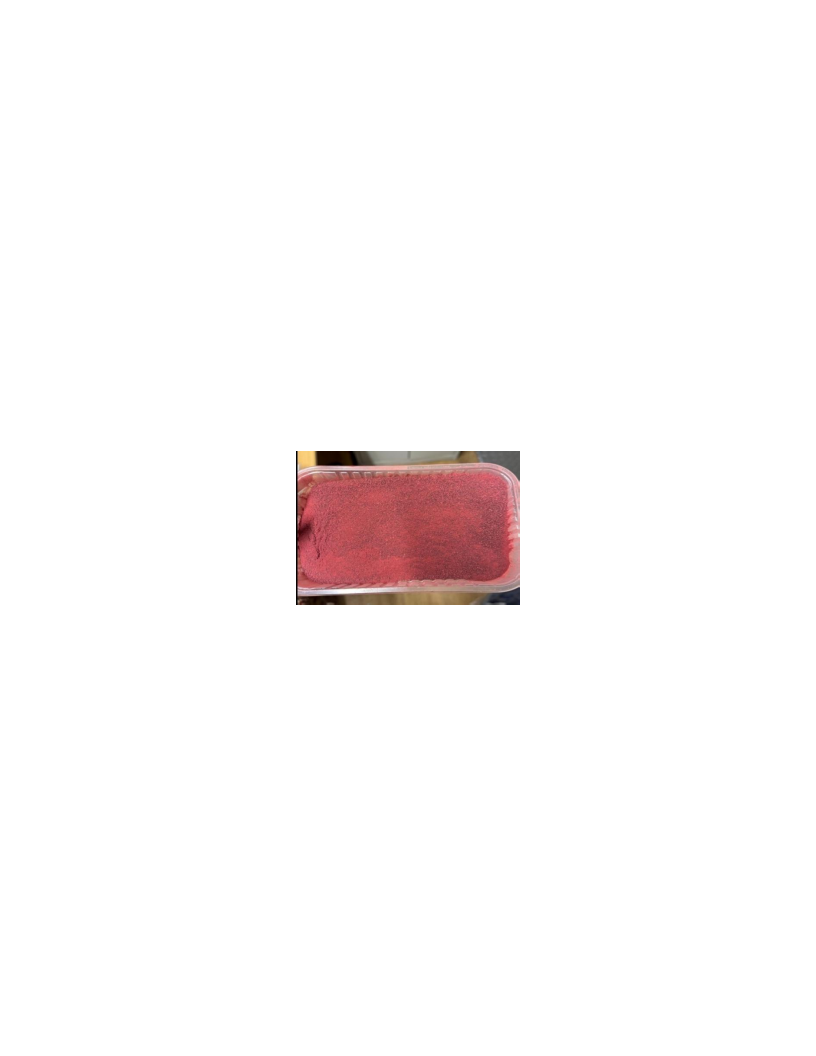
\includegraphics[width=0.8\textwidth]{media/pish3/image7}
	\caption*{}
\end{figure}


{\bfseries 1- сурет. Құрғақ қызылша ұнтағы}

Тәжірибелік йогурт үлгілері термостаттық әдіспен алынды. Алдын ала
аналитикалық таразыда 0,1, 0,25 және 0,5 г массасындағы қызылша
ұнтағының үш өлшемі және әрқайсысы 1 г болатын ашытқының төрт өлшемі
өлшенді.

{\bfseries 2- кесте.Йогурт дайындаудыңрецептурасы}

% \begin{longtable}[]{@{}
%   >{\raggedright\arraybackslash}p{(\columnwidth - 6\tabcolsep) * \real{0.1482}}
%   >{\raggedright\arraybackslash}p{(\columnwidth - 6\tabcolsep) * \real{0.2593}}
%   >{\raggedright\arraybackslash}p{(\columnwidth - 6\tabcolsep) * \real{0.3892}}
%   >{\raggedright\arraybackslash}p{(\columnwidth - 6\tabcolsep) * \real{0.2033}}@{}}
% \toprule\noalign{}
% \multirow{2}{=}{\begin{minipage}[b]{\linewidth}\raggedright
% \end{minipage}} &
% \multicolumn{3}{>{\raggedright\arraybackslash}p{(\columnwidth - 6\tabcolsep) * \real{0.8518} + 4\tabcolsep}@{}}{%
% \begin{minipage}[b]{\linewidth}\raggedright
% 1 тонна өнімге
% \end{minipage}} \\
% & \begin{minipage}[b]{\linewidth}\raggedright
% сүт
% \end{minipage} & \begin{minipage}[b]{\linewidth}\raggedright
% қызылша ұнтағы
% \end{minipage} & \begin{minipage}[b]{\linewidth}\raggedright
% қант
% \end{minipage} \\
% \midrule\noalign{}
% \endhead
% \bottomrule\noalign{}
% \endlastfoot
% 0 & 97 & - & 3\% \\
% 1 & 96,9 & 0,1\% & 3\% \\
% 2 & 96,75 & 0,25\% & 3\% \\
% 3 & 96,5 & 0,5\% & 3\% \\
% \end{longtable}

Сүтті қабылдау

Тазалау, салқындату (t=4-6⁰C)

Жылыту (t=38-40⁰С)

Нормалау, араластыру (t=38-40⁰C)

Гомогендеу (t=55-60⁰C,р=15-17мПа)

Ұнтақтау

Пастерлеу (t=93-95⁰C)

Салқындату
\begin{figure}[H]
	\centering
	
\includegraphics[width=0.8\textwidth]{media/pish3/image8}
	\caption*{}
\end{figure}


Ұйытқы қосу, араластыру (10-15мин)

Ұйыту (t=37-38⁰C, pH=4,6)

Салқындату, араластыру (t=21-22⁰C)

Буып, түю

Сақтау (t=4-6⁰C)

Сатылымға жіберу

{\bfseries 2- сурет. Йогурт дайындау технологиясы.}

Йогурт дайындау бірнеше кезеңнен тұрды (2-сурет):

- алдын ала сүт электр плитасында 80 °C температурада 10 минут бойы
қосымша пастерленді. Кейінгі барлық процестер микробиологиялық
қауіпсіздік боксында стерильді жағдайда жүргізілді.

- алдын ала дайындалған стерильді шыны ыдыстарға өлшегіш цилиндрдің
көмегімен 1 л дайындалған сүт құйылды. Әр ыдысқа тиісті мөлшердегі
қызылша ұнтағы қосылып, бір ыдысқа қызылша ұнтағы енгізілмеді (бақылау
үлгісі). Өсімдік текті қоспа енгізілгеннен кейін сүт қоспалары мұқият
араластырылды, содан кейін ашытқының алдын ала дайындалған өлшемдері
қосылып, қайтадан араластырылды. Банкілердің қақпақтары мықтап жабылды.

- ферментация табиғи ауа айналымы бар термостатта 37-38 °C температурада
жүргізілді. Ферментация процесі термостаттық әдіспен жүргізіліп,
нәтижесінде йогурттың ұю уақыты 10 сағатты құрады. Дайын өнімнің
құрылымын тұрақтандыру және сақтау мерзімін ұзарту мақсатында, йогурт
үлгілері +4 °C температурадағы салқындатқыш камерасына қойылды.

Осылайша, келесі йогурт үлгілері алынды:

-бақылау үлгісі - дәстүрлі технология бойынша дайындалған, қызылша
ұнтағы қосылмаған йогурт;

- 1-үлгі - өнім массасына шаққанда 0,1 \% мөлшерінде қызылша ұнтағы
қосылған йогурт;

{\bfseries -} 2-үлгі - өнім массасына шаққанда 0,25 \% мөлшерінде қызылша
ұнтағы қосылған йогурт;

{\bfseries -} 3-үлгі - өнім массасына шаққанда 0,5 \% мөлшерінде қызылша
ұнтағы қосылған йогурт;

Алынған йогурт үлгілерінің сапасын бақылау сақтау мерзімінің 3-ші
тәулігінде жүргізілді. Талдау барысында келесі көрсеткіштер анықталды:

{\bfseries -} органолептикалық көрсеткіштер (3-кесте) -- сыртқы түрі мен
консистенциясы, дәмі мен иісі, түсі ГОСТ 31981-2013 {[}9{]} стандартының
талаптарына сәйкес бағаланды. Сонымен қатар, 6 ерікті қатысушының
қатысуымен йогурт үлгілерінің органолептикалық қасиеттерін бағалау
мақсатында дәмін сынау жүргізілді;

{\bfseries -} физика-химиялық көрсеткіштер (4-кесте) -- ГОСТ 3624-92
{[}10{]} стандартына сәйкес қышқылдық деңгейі, құрғақ заттардың мөлшері,
тығыздығы, темірдің массалық үлесі анықталды.

{\bfseries Нәтижелері және талқылау.} Жүргізілген зерттеулер нәтижесінде
алынған йогурт үлгілерінің барлығы органолептикалық, физико-химиялық
және микробиологиялық көрсеткіштері бойынша ГОСТ 31981-2013 {[}11{]}
талаптарына сәйкес келетіні анықталды.

Йогуртқа қызылша ұнтағын қосу оның барлық органолептикалық
сипаттамаларына әсер етті (3-кесте). Өсімдік негізіндегі тағамдық
қоспаны 0,25 \% мөлшерінде қолдану йогурттың сыртқы көрінісін,
текстурасы мен консистенциясын жақсартып, сарысу бөлінуін азайтты.
Қызылша қосылған йогурттар жағымды қызғылт түске ие болды, бұл
дегустация кезінде респонденттер тарапынан ерекше атап өтілді.

Дегустация нәтижелері бойынша ең жоғары бағаны қызылша концентрациясы
0,25 \% болған № 2 үлгісі алды (3-кесте). Ал ең төменгі баға 0,5\%
қызылша ұнтағы қосылған № 3 үлгісіне берілді.

{\bfseries 3- кесте.Үлгілердің органолептикалық көрсеткіштері}

% \begin{longtable}[]{@{}
%   >{\raggedright\arraybackslash}p{(\columnwidth - 8\tabcolsep) * \real{0.2205}}
%   >{\raggedright\arraybackslash}p{(\columnwidth - 8\tabcolsep) * \real{0.2110}}
%   >{\raggedright\arraybackslash}p{(\columnwidth - 8\tabcolsep) * \real{0.1912}}
%   >{\raggedright\arraybackslash}p{(\columnwidth - 8\tabcolsep) * \real{0.2058}}
%   >{\raggedright\arraybackslash}p{(\columnwidth - 8\tabcolsep) * \real{0.1715}}@{}}
% \toprule\noalign{}
% \multirow{4}{=}{\begin{minipage}[b]{\linewidth}\raggedright
% Көрсеткіштер
% \end{minipage}} &
% \multicolumn{4}{>{\raggedright\arraybackslash}p{(\columnwidth - 8\tabcolsep) * \real{0.7795} + 6\tabcolsep}@{}}{%
% \begin{minipage}[b]{\linewidth}\raggedright
% Үлгі
% \end{minipage}} \\
% & \begin{minipage}[b]{\linewidth}\raggedright
% бақылау
% \end{minipage} & \begin{minipage}[b]{\linewidth}\raggedright
% №1
% \end{minipage} & \begin{minipage}[b]{\linewidth}\raggedright
% №2
% \end{minipage} & \begin{minipage}[b]{\linewidth}\raggedright
% №3
% \end{minipage} \\
% &
% \multicolumn{4}{>{\raggedright\arraybackslash}p{(\columnwidth - 8\tabcolsep) * \real{0.7795} + 6\tabcolsep}@{}}{%
% \begin{minipage}[b]{\linewidth}\raggedright
% Қызылша концентрациясы
% \end{minipage}} \\
% & \begin{minipage}[b]{\linewidth}\raggedright
% 0,00
% \end{minipage} & \begin{minipage}[b]{\linewidth}\raggedright
% 0,1
% \end{minipage} & \begin{minipage}[b]{\linewidth}\raggedright
% 0,25
% \end{minipage} & \begin{minipage}[b]{\linewidth}\raggedright
% 0,5
% \end{minipage} \\
% \midrule\noalign{}
% \endhead
% \bottomrule\noalign{}
% \endlastfoot
% Сыртқы түрі & біртекті, қою ұйытындысы бар, аз мөлшерде сарысу бөлінген
% & біртекті, қою ұйытындысы бар, сарысу бөлінбеген, крем тәрізді текстура
% & біртекті, қою ұйытындысы бар, сарысу бөлінбеген, крем тәрізді текстура
% & біртекті, қою ұйытындысы бар, көп мөлшерде сарысу бөлінген \\
% Дәмі, исі & таза қышқыл-сүтті & аздап қышқыл, тәттілеу & аздап қышқыл,
% тәттілеу & қышқыл, қызылшаға тән айқын дәмі мен иісі бар \\
% Түсі & сүттей ақ, біртекті & бозғылт қызғылт, біртекті & бозғылт
% қызғылт, біртекті & қызғылт, біртекті \\
% Дегустацияның қорытынды бағасы & 4,75 & 4,86 & 4,96 & 4,53 \\
% \end{longtable}

Йогурт үлгілерінің тағамдық құндылығының өзгерістерін есептеу нәтижелері
бойынша, қызылша ұнтағы қосылған №2 үлгіде адам ағзасы үшін аса маңызды
минерал -- темірдің мөлшері өзгергені анықталды.

Теориялық есептеулерді растау үшін темір мөлшеріне талдау жүргізілді:
бақылау үлгісі мен қызылша ұнтағының орташа мөлшері бар №1, №2 үлгі
зерттелді.

Қызылшаның құрамында органикалық қышқылдар бар, сондықтан қызылша ұнтағы
сүтке қосылғанда, рН көрсеткіші төмендейді (4-кесте){\bfseries .}

{\bfseries 4-кесте. Үлгілердің физика-химиялық көрсеткіштері}

% \begin{longtable}[]{@{}
%   >{\raggedright\arraybackslash}p{(\columnwidth - 8\tabcolsep) * \real{0.3144}}
%   >{\raggedright\arraybackslash}p{(\columnwidth - 8\tabcolsep) * \real{0.1085}}
%   >{\raggedright\arraybackslash}p{(\columnwidth - 8\tabcolsep) * \real{0.1218}}
%   >{\raggedright\arraybackslash}p{(\columnwidth - 8\tabcolsep) * \real{0.1236}}
%   >{\raggedright\arraybackslash}p{(\columnwidth - 8\tabcolsep) * \real{0.3316}}@{}}
% \toprule\noalign{}
% \multirow{2}{=}{\begin{minipage}[b]{\linewidth}\raggedright
% Көрсеткіш
% 
% атаулары
% \end{minipage}} &
% \multicolumn{3}{>{\raggedright\arraybackslash}p{(\columnwidth - 8\tabcolsep) * \real{0.3540} + 4\tabcolsep}}{%
% \begin{minipage}[b]{\linewidth}\raggedright
% Үлгілер
% \end{minipage}} &
% \multirow{2}{=}{\begin{minipage}[b]{\linewidth}\raggedright
% Нормативтік көрсеткіштер
% \end{minipage}} \\
% & \begin{minipage}[b]{\linewidth}\raggedright
% 1
% \end{minipage} & \begin{minipage}[b]{\linewidth}\raggedright
% 2
% \end{minipage} & \begin{minipage}[b]{\linewidth}\raggedright
% 3
% \end{minipage} \\
% \midrule\noalign{}
% \endhead
% \bottomrule\noalign{}
% \endlastfoot
% Қышқылдылық, °Т & 135,0 & 110,0 & 105,0 & 75,0-140,0 \\
% Тығыздығы, \% & 31,98 & 35,6 & 44,27 & рецептура бойынша \\
% Құрғақ заттарының жалпы мөлшері, \% аз емес & 9,79 & 10,0 & 12,05 &
% компоненттерсіз 9,5
% 
% компоненттермен 8,5 \\
% Темірдің массалық үлесі, мк/кг, көп емес & 0,0 & 0,0 & 0,1786 &
% -\/-\/-\/-\/-\/-\/- \\
% \end{longtable}

Зерттелген тағамдық қоспаны пайдалану йогурттың физико-химиялық
көрсеткіштеріне, құрамында темір мөлшерінің жоғарылауына оң әсер етті.
(4-кесте). Қызылша ұнтағы қосылған үлгілерде синерезис деңгейі төмендеп,
керісінше, су байланыстыру қабілеті артты. Бұл олардың сыртқы түріне де
әсер етті: № 2--3 үлгілерінің тығыздығы мен тұтқырлығы жоғары болды
(4-кесте) және олар жағымды текстураға ие болды.

Алайда, 0,5 \% қызылша ұнтағы қосылған № 3 үлгісінде кері әсер байқалды.
Бұл өнімнің сыртқы көрінісі тартымды болғанмен, дәмі мен иісінде
қызылшаның өткірлігі байқалады.

Зерттелген үлгілердің құрғақ қалдығы енгізілген тағамдық қоспа мөлшеріне
байланысты өзгерді: өнімдегі қызылша ұнтағының концентрациясы артқан
сайын, бұл көрсеткіш те жоғарылады (4-кесте).

Барлық үлгілердегі титрленетін қышқылдық көрсеткіші (4-кесте) ГОСТ
31981-2013 {[}11{]} талаптарына сәйкес рұқсат етілген шектерде болды.

{\bfseries Қорытынды.} Жүргізілген зерттеулер нәтижесінде өсімдік
компоненттерімен байытылған және ГОСТ 31981 талаптарына жауап беретін
сүт қышқылы өнімі алынды {[}11{]}. Сонымен қатар, йогурт дайындау
кезінде қызылшаны пайдалану оның тағамдық құндылығын және құрамындағы
темірдің мөлшерін арттырады деген қорытынды жасауға болады. Қызылша
ұнтағының оңтайлы мөлшері 0,25\% деп анықталды. Мұндай көлемдегі
қызылшасы бар йогурттар түсі, дәмі, иісі және консистенциясы жағымды,
физикалық-химиялық көрсеткіштері бақылау үлгісінен жоғары. Ұнтаққа
қызылшаның аз мөлшерін қосу тиімді емес, өйткені ол тағамдық құндылығын
немесе дәмін айтарлықтай өзгертпейді. Қызылша ұнтағының жоғары
концентрациясы йогурттың органолептикалық және физика-химиялық
қасиеттерінің нашарлауына әкеледі.

{\bfseries Әдебиеттер}

1.Karnopp A. R. et al. Optimization of an organic yogurt based on
sensorial, nutritional, and functional perspectives //Food Chemistry.-
2017.-Vol.233.-P.401-411.

DOI 10.1016/j.foodchem.2017.04.112

2.Abdi-Moghadam Z. et al. Functional yogurt, enriched and probiotic: A
focus on human health //Clinical nutrition ESPEN.
-2023.-Vol.57.-P.575-586

DOI 10.1016/j.clnesp.2023.08.005

3.Scalbert A., Johnson I.T., \& Saltmarsh M. (2005). Polyphenols:
antioxidants and beyond//The American Journal of Clinical
Nutrition.-2005.-Vol. 81(1).-P. 215-217.

DOI 10.1093/ajcn/81.1.215S

4.Семен З. Антиоксиданты--природный щит здоровья человека (Antioxidants
are a natural shield of human health). Дата обращения:24.12.2024.

\href{https://www.netanyascientific.com/Stati/Stati-5/data/Zlatin_Antioxidants.pdf5.Dong-5.Dong}{https://www.netanyascientific.com/Stati/Stati-5/data/Zlatin\_Antioxidants.pdf5.Dong-5.Dong}
Ping Xu, Ya Li, Xiao Meng, et al. Natural Antioxidants in Foods and
Medicinal Plants: Extraction, Assessment and Resources// Int. J. Mol.
Sci\emph{.}~-2017.-Vol.~18(1)
\href{https://doi.org/10.3390/ijms18010096}{DOI 10.3390/ijms18010096}

6.Голубев А. А., Дунченко Н. И., Купцова С. В. Пищевые потери и роль
натуральных. Aнтиоксидантов в решении этой проблемы:
анализ~и~перспективы// Молочная промышленность.-2024.- №1.-C.40-45. DOI
10.21603/1019-8946-2024-1-9

7.Fan X. et al. The effect of natural plant-based homogenates as
additives on the quality of yogurt: A review //Food
Bioscience.-2022.-Vol.49:101953

101953. DOI10.1016/j.fbio.2022.101953

8.
\href{https://ascidatabase.com/author.php?ascicat=ALL&author=S.U.&mid=&last=Wisam}{S.U.
Wisam},~\href{https://ascidatabase.com/author.php?ascicat=ALL&author=T.K.&mid=&last=Nahla}{T.K.
Nahla}~and~\href{https://ascidatabase.com/author.php?ascicat=ALL&author=N.M.&mid=&last=Tariq}{N.M.
Tariq} Antioxidant activities of beetroot (Beta vulgaris L.) extracts.//
\href{https://www.researchgate.net/journal/Pakistan-Journal-of-Nutrition-1680-5194?_tp=eyJjb250ZXh0Ijp7ImZpcnN0UGFnZSI6InB1YmxpY2F0aW9uIiwicGFnZSI6InB1YmxpY2F0aW9uIn19}{Pakistan
Journal of Nutrition}.-2024.-Vol.17(10).-P.500-505~

DOI 10.3923/pjn.2018.500.505

9.Бахарев В. В. и др. Исследование физико-химических показателей
свекольных выжимок после их дегидратации с последующей экструзией
//Индустрия питания/Food Industry.-2022. -Т.7.(3).- С.25-31. DOI
10.29141/2500-1922-2022-7-3-3

10.ГОСТ 3624-92. Молоко и молочные продукты. Титриметрические методы
определения кислотности. Введ. 1994-01-01. М.: ИПК Изд-во стандартов,
2004.

11.ГОСТ 31981-2013. Йогурты. Общие технические условия. т. Введ.
2014-05-01. М.: Стандартинформ, 2014.

{\bfseries References}

1.Karnopp A. R. et al. Optimization of an organic yogurt based on
sensorial, nutritional, and functional perspectives //Food Chemistry.-
2017.-Vol.233.-P.401-411.

DOI 10.1016/j.foodchem.2017.04.112

2.Abdi-Moghadam Z. et al. Functional yogurt, enriched and probiotic: A
focus on human health //Clinical nutrition ESPEN.
-2023.-Vol.57.-P.575-586

DOI 10.1016/j.clnesp.2023.08.005

3.Scalbert A., Johnson I.T., \& Saltmarsh M. (2005). Polyphenols:
antioxidants and beyond//The American Journal of Clinical
Nutrition.-2005.-Vol. 81(1).-P. 215-217.

DOI 10.1093/ajcn/81.1.215S

4.Semen Z. Antioksidanty--prirodnyj shhit zdorov' ja
cheloveka (Antioxidants are a natural shield of human health). Data
obrashhenija:24.12.2024.

\url{https://www.netanyascientific.com/Stati/Stati-5/data/Zlatin_Antioxidants.pdf5.Dong-}

\href{https://www.netanyascientific.com/Stati/Stati-5/data/Zlatin_Antioxidants.pdf5.Dong-5.Dong}{5.Dong}
Ping Xu, Ya Li, Xiao Meng, et al. Natural Antioxidants in Foods and
Medicinal Plants: Extraction, Assessment and Resources// Int. J. Mol.
Sci\emph{.}~-2017.-Vol.~18(1)
\href{https://doi.org/10.3390/ijms18010096}{DOI 10.3390/ijms18010096}

6.Golubev A. A., Dunchenko N. I., Kupcova S. V. Pishhevye poteri i
rol'{} natural' nyh. Antioksidantov v
reshenii jetoj problemy: analiz i perspektivy// Molochnaja
promyshlennost'.-2024.- №1.-C.40-45. DOI
10.21603/1019-8946-2024-1-9

7.Fan X. et al. The effect of natural plant-based homogenates as
additives on the quality of yogurt: A review //Food
Bioscience.-2022.-Vol.49:101953

101953. DOI10.1016/j.fbio.2022.101953

8.
\href{https://ascidatabase.com/author.php?ascicat=ALL&author=S.U.&mid=&last=Wisam}{S.U.
Wisam},~\href{https://ascidatabase.com/author.php?ascicat=ALL&author=T.K.&mid=&last=Nahla}{T.K.
Nahla}~and~\href{https://ascidatabase.com/author.php?ascicat=ALL&author=N.M.&mid=&last=Tariq}{N.M.
Tariq} Antioxidant activities of beetroot (Beta vulgaris L.) extracts.//
\href{https://www.researchgate.net/journal/Pakistan-Journal-of-Nutrition-1680-5194?_tp=eyJjb250ZXh0Ijp7ImZpcnN0UGFnZSI6InB1YmxpY2F0aW9uIiwicGFnZSI6InB1YmxpY2F0aW9uIn19}{Pakistan
Journal of Nutrition}.-2024.-Vol.17(10).-P.500-505~

DOI 10.3923/pjn.2018.500.505

10.GOST 3624-92. Moloko i molochnye produkty. Titrimetricheskie metody
opredeleniya kislotnosti. Vved. 1994-01-01. M.: IPK Izd-vo standartov,
2004.

11.GOST 31981-2013. Yogurty. Obshchie tekhnicheskie usloviya. Vved.
2014-05-01. M.: Standartinform, 2014.

\emph{{\bfseries Авторлар туралы мәліметтер}}

Машанова Н.С{\bfseries .}- доктор технических наук, КАТИУ атындағы С.
Сейфуллина,Астана Казахстан, е-mail:
\href{mailto:nurmashanova@gmail.com}{\nolinkurl{nurmashanova@gmail.com}}.
ORCID: https://orcid.org/0000-0001-8664-5173;

Калемшарив Б. - КАТИУ атындағы С. Сейфуллина, Астана Қазақстан; е-mail:
begjan.ae@gmail.com \url{https://orcid.org/0000-0002-8036-9718}

Жолшиева А.С.-техника ғылымдарының магистрі, С. Сейфуллин атындағы
КазАТЗУ, Астана Қазақстан,е-mail: aksamal\_96@mail.ru
\url{https://orcid.org/0009-0002-9232-782X}

Бектурганова А.А.- техника ғылымдарының кандитаты, асс.профессор,Қ.К.
Құлажанов атындағы Қазақ технология және бизнес университеті, Астана,
Қазақстан, е-mail:
\href{mailto:1968al1@mail.ru}{\nolinkurl{1968al1@mail.ru}}
\url{https://orcid.org/0000-0002-0906-2027}

\emph{{\bfseries Information about the authors}}

Mashanova N.- Doctor of Technical Sciences, Senior lecturer, at
S.Seifullin KATSU, Astana, Kazakhstan, e-mail: nurmashanova@gmail.com;

Kalemshariv B.- master of engineering, at.Seifullin KATSU, Astana,
Kazakhstan; e-mail: begjan.ae@gmail.com;

Zholshiyeva A - Master of Technical Sciences, S.Seifullin KATSU, Astana,
Kazakhstan, e-mail: aksamal\_96@mail.ru;

Bekturganova A.A. - Candidate of Technical Sciences, Assistant
Professor,Kazakh University of Technology and Business named after K.
Kulazhanov, Astana, Kazakhstan, е-mail: 1968al1@mail.ru